\section{Theory}
\label{sec:theory}

\subsection{Rigid body kinematics}
\label{sec:kinematics}
We describe the body with two frames: a lab frame fixed in space, and a body frame with axes $\vb{e}_1,\vb{e}_2,\vb{e}_3$ that rotate with the body.
The rotation is described by the angular velocity $\vb*{\omega}$, and each body axis moves as $\dot{\vb{e}}_k=\vb*{\omega}\times\vb{e}_k$.
We write $\Omega_k=\vb*{\omega}\vdot\vb{e}_k$ for the components of $\vb*{\omega}$ in the body frame.
For a free body no torque acts, so the angular momentum $\vb{L}$ is fixed in the lab frame.
Seen from the body, however, $\vb{L}$ moves, and following this motion is the key to the effect.

\subsection{The inertia tensor}
\label{sec:inertia}
For a body made of point masses $m_i$ at positions $\vb{r}_i$ from the centre of mass, the inertia tensor is
\begin{equation}
    I_{ab} = \sum_i m_i\left(r_i^2\,\delta_{ab} - r_{i,a}\,r_{i,b}\right)
    \label{eq:inertia}
\end{equation}
and $\vb{L}=\mathsf{I}\,\vb*{\omega}$.
In general $\vb{L}$ and $\vb*{\omega}$ are not parallel.
Since $\mathsf{I}$ is symmetric, there are three perpendicular \emph{principal axes} in which it is diagonal, with principal moments $I_1>I_2>I_3$.
Spinning about any one of them keeps $\vb{L}$ parallel to $\vb*{\omega}$.
Our main body is an octahedron of six \SI{1}{kg} masses at $(\pm1,0,0)$, $(0,\pm2,0)$ and $(0,0,\pm3)$\,m, whose principal axes are $x$, $y$ and $z$ with $I_x=26$, $I_y=20$ and $I_z=\SI{10}{kg.m^2}$, so $y$ is the middle axis.

\subsection{Euler's equations}
\label{sec:euler}
Written in the body frame along the principal axes, $\dot{\vb{L}}=0$ becomes Euler's equations,
\begin{equation}
\begin{aligned}
    I_1\dot\Omega_1 &= (I_2 - I_3)\,\Omega_2\Omega_3\\
    I_2\dot\Omega_2 &= (I_3 - I_1)\,\Omega_3\Omega_1\\
    I_3\dot\Omega_3 &= (I_1 - I_2)\,\Omega_1\Omega_2
\end{aligned}
\label{eq:euler}
\end{equation}
They conserve the kinetic energy and the magnitude of the angular momentum,
\begin{equation}
    2E = \sum_k \frac{L_k^2}{I_k},\qquad L^2 = \sum_k L_k^2,
    \label{eq:conserved}
\end{equation}
with $L_k=I_k\Omega_k$.
These two quantities are what we monitor to check our simulations (\cref{sec:conservation}).

\subsection{Instability of the middle axis}
\label{sec:stability}
Suppose the body spins with rate $\Omega$ about one principal axis and is given a small tilt.
It can be shown that about the axes of largest and smallest moment the tilt only oscillates, but about the intermediate axis it grows as $e^{\lambda t}$ with
\begin{equation}
    \lambda = \Omega\sqrt{\frac{(I_1-I_2)(I_2-I_3)}{I_1 I_3}}.
    \label{eq:lambda}
\end{equation}
For the octahedron this gives $\lambda\approx0.480\,\Omega$.
If the initial tilt has size $\varepsilon$, it becomes of order one, which is a flip, after roughly
\begin{equation}
    t_{\text{flip}} \approx \frac{1}{\lambda}\ln\frac{1}{\varepsilon},
    \label{eq:tflip}
\end{equation}
so the flip time grows only slowly as the tilt is made smaller.
We test this in \cref{sec:res-fliptime}.

\subsection{Geometric picture: the polhode}
\label{sec:polhode}
\Cref{eq:conserved} gives a simple picture of the motion.
In the body frame $\vb{L}$ must lie on a sphere of radius $L$ and, at the same time, on the energy ellipsoid.
It therefore moves along the curve where the two surfaces meet, called the polhode (\cref{fig:polhode-family}).
Near the largest and smallest axes these curves are small closed loops, so $\vb{L}$ stays close to the axis and the rotation is stable.
Near the middle axis the two surfaces cross, and the special curve through this axis, the separatrix, carries $\vb{L}$ all the way to the opposite side.
\begin{figure}[H]
    \centering
    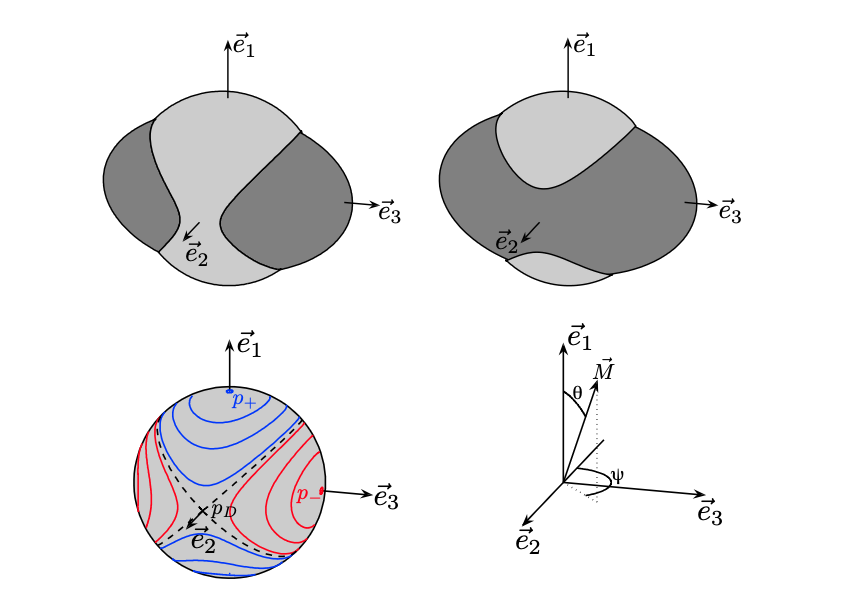
\includegraphics[width=\linewidth]{Images/polhode_vandamme.png}
    \caption{Top: the energy ellipsoid (dark) and the angular momentum sphere (light). Bottom left: polhodes on the sphere, with the separatrix dashed. Adapted from \cite{vandamme2017}.}
    \label{fig:polhode-family}
\end{figure}
